\documentclass{article}

% if you need to pass options to natbib, use, e.g.:
%     \PassOptionsToPackage{numbers, compress}{natbib}
% before loading neurips_2018

% ready for submission
% \usepackage{neurips_2018}

% to compile a preprint version, e.g., for submission to arXiv, add add the
% [preprint] option:
%     \usepackage[preprint]{neurips_2018}

% to compile a camera-ready version, add the [final] option, e.g.:
     \usepackage[final]{nips}

% to avoid loading the natbib package, add option nonatbib:
%     \usepackage[nonatbib]{neurips_2018}
\usepackage{graphicx}
\usepackage[utf8]{inputenc} % allow utf-8 input
\usepackage[T1]{fontenc}    % use 8-bit T1 fonts
\usepackage{hyperref}       % hyperlinks
\usepackage{url}            % simple URL typesetting
\usepackage{booktabs}       % professional-quality tables
\usepackage{amsfonts}       % blackboard math symbols
\usepackage{nicefrac}       % compact symbols for 1/2, etc.
\usepackage{microtype}      % microtypography

\title{Movie Rating Prediction Using Machine Learning}

% The \author macro works with any number of authors. There are two commands
% used to separate the names and addresses of multiple authors: \And and \AND.
%
% Using \And between authors leaves it to LaTeX to determine where to break the
% lines. Using \AND forces a line break at that point. So, if LaTeX puts 3 of 4
% authors names on the first line, and the last on the second line, try using
% \AND instead of \And before the third author name.

\author{%
  Grigor ~Keropyan\thanks{https://github.com/grigor97} \\
  Department of Mathematics and Mechanics\\
  Yerevan State University\\
  \texttt{goqorkeropyan@gmail.com} \\
}

\begin{document}
% \nipsfinalcopy is no longer used

\maketitle

\begin{abstract}
  Movie rating prediction based on information available prior to theatrical release is important in order to understand how successful will be movie. This paper describes various Machine Learning methods to predict movie rating. 
\end{abstract}

\section{Introduction}

Movie rating prediction is becoming a popular problem and various methods have been suggested. In this paper we will introduce Machine Learning (ML) methods to predict movie rating based on the data available prior to the theatrical release. We used IMDB open-source data such as posters and run-time of movies. \\

Although, it seems impossible to predict the movie rating based on the information available before theatrical release, we will see that ML methods predict them quite accurately. One of the explanation could be that people may like movies if their preferred actor is in the crew or films are produced by their favorite producers.\\

One of the goals of this work is provide a tool which can help producers to promote their films to be successful. Another one is that this work provide a good recommendation for people predicting their IMDB score. 

\section{Related Work}
\label{rel_work}

This work is based on the Stanford students paper [1] where they predict IMDB score of movies. In [1] authors used ML based methods to predict IMDB score. Another research which uses Bayesian approach [2]. This paper is based on [1] and uses new ML algorithms such as lightgbm to reach the better accuracy than [1]. Our preproccessing is almost the same as [1] and we have about 20K examples. We have shuffled the dataset and splited into training and test test correspondingly 80 and 20 precents. In the algorithm we have done K-Folds cross validation and after tuning the hyperparamters we have achieved better accuracy than [1]. 

\section{Dataset and Features}
\label{headings}

We have used open source data, "Movie Genre from its Poster Dataset" [3] and "The Movie Dataset" [4]. The dataset is preprocessed like [1], taking only movies which original language is english and which produced after 1980. The features are divided into 3 groups: text (synopses), images (posters) and others (runtime, genre, director, actors). From poster we have extracted some features: such as number of peoples in the poster, mean and standard deviation of blue, green, red, hue, saturation, brightness as in [5]. For summaries we have used count vectorizers and only left the word which appeared more than 20 times. Directors are have been made one hot and actors count vectorizers where we have only left top three actors in each movie. The example of result is shown in Table 1. 

\begin{table}
  \caption{Dataset by Groups}
  \label{dataset-table}
  \centering
  \begin{tabular}{llll}
    \toprule
    Data & Type & Dimension & Example  \\
    \midrule
    Actors & Categorical  & 1671 &  Tom Hanks   \\
    poster & Numerical & 13 & Number of faces = 0 \\
    Director & Categorical & 491 & Howard Deutch \\
    Runtime & Numerical & 1 & 121 (minutes) \\
    Genre & Categorical & 23 & Documentation \\
    Synopses & Categorical & 3712 & Once \\
    \bottomrule
  \end{tabular}
\end{table}
After filtering the english movies and released after 1980 it remained 18850 movies. Which we have splited in two ways. First: like [1] implementation, when it is separated train, validation and test sets correspondingly 70, 15, 15 percents. Second: which gave a better result it is separated into train and test sets correspondingly 80 and 20 percents. 

\section{Methods}
\label{methods}

In this chapter we will speak about the models which have been tried for the dataset. 

\subsection{Linear Regression}

Linear Regression (LR) is on e of the widely used ML algorithms. It is simple and performs well in many tasks. LR discovers linear relationship between input and target data. In many real world applications target is actually linearly dependent of the input data. So, in this problems LR is a good choice. 

In order to avoid overfitting we have also used Ridge Regressor. For this dataset latter one performed better than the former one. The reason could be that in that dataset exist outliers which deviate LR to perform well. Using the regularization model performed sagnificantly better. 


\subsection{Decision Tree and Random Forest}

Decision Trees and Random Forests are commonly used interpretable models. Decision Tree model in each point of tree divides some feature in order to maximize targeted loss function. Random Forest is an assemble of Decision Trees which could perform better in complex data case. 

As we will see in the next section Random Forest performed better than LR. The reason is that we have a a lot of categorical features which is more easy for Random Forest to separate from each other. 


\subsection{XGBoost}

XGBoost is a new model compared with former ones. This model also an assemble of trees, but it adds regularization term to the loss function and uses another technique to find an optimal solution. 

XGBoost also performed well on the dataset and it is better than LR models. Actually, Without fine tuning it performed a little worse than Random Forest. 

\subsection{Support Vector Regressor}

Support Vector Machine is widely used ML algorithm which performs well in many problems. It defines a margin between points and only points beyond the margin affect on the loss. SVR instead, defines a margin of epsilon-distance and points inside the boundaries of regions do not affecting to loss. 

\subsection{Lightgbm}

Lightgbm is based on XGBoost and it performs better than XGBoost in many tasks. It also very fast algorithm. We have used this model and after fine tuning it produces the best result. It outperforms to the results in [1] sagnificantly. 

\subsection{Classification}
We have also tried classification for IMDB score prediction. The score is discretized by 5, 10 and 20 classes and same models beside Lightgbm we have tried for classification problem. As we will see in the next section, for any model classification test MSE is larger than regression test MSE.

\section{Experiments and Results}

As in [1] we have also used Mean Squared Error (MSE) and $R^2$ as our metrics. MSE is also used for hyperparameter tuning and $R^2$ for getting some information about the performance of models comparing with other models. 

In many of the models we have tested them like in [1] by separating train, validation and test sets. Then found a best model according to the validation set and finally testing it in test set. That models result you can see in Table 2. IN this models the best one is Random Forest. After parameter tuning it achieved 0.44 $R^2$ score which is better than the best score in [1]. 

\begin{table}
  \caption{Train Validation Test Results}
  \label{tvt_results-table}
  \centering
  \begin{tabular}{lll}
    \toprule
    Method & Test MSE &  Test $R^2$  \\
    \midrule
    Linear Regression & 1.3918  & 0.0668   \\
    Ridge Regression & 0.9824  & 0.3413   \\
    Decision Tree & 0.9153  & 0.3863   \\
    Random Forest & 0.8290  & 0.4441   \\
    XGBoost & 0.8375 & 0.4384 \\
    SVR & 0.9294 & 0.3768 \\
        \bottomrule
  \end{tabular}
\end{table}


Another approach is held using Lightgbm model with Hyperopt hyperparameter tuning algorithms. In this model we have separated just train and test sets 80 and 20 percents correspondingly. And using Hyperopt lightgbm model achieved 0.45 $R^2$ accuracy which is better than previous best model. It is worth to consider that in this case test data is sagnificantly more than in previous case as we have taken 20 percent of the whole dataset. The result is shown in Table 3.

\begin{table}
  \caption{Lightgbm Result}
  \label{lgb_results-table}
  \centering
  \begin{tabular}{lll}
    \toprule
    Method & Test MSE &  Test $R^2$  \\
    \midrule
    Lightgbm & 0.8067  & 0.4513   \\
        \bottomrule
  \end{tabular}
\end{table}

In Table 4 you can see comparison with results of [1]. It can be seen that [1] performed better in the case of LR, Decision Tree, Ridge Regression and SVR. The reason is that we have not done parameter tuning on this models. However in the case of Random Forest our accuracies outperform all their results. 

\begin{table}
  \caption{Comparison with [1]}
  \label{cmp_results-table}
  \centering
  \begin{tabular}{lllll}
    \toprule
    Method & our MSE & [1] MSE &  our $R^2$  & [1] $R^2$  \\
    \midrule
    Linear Regression & 1.3918 & 0.9302  & 0.0668  & 0.3745   \\
    Ridge Regression & 0.9824 & 0.8775  & 0.3413 & 0.4099  \\
    Decision Tree & 0.9153  & 0.8959 & 0.3863  & 0.3975 \\
    Random Forest & 0.8290  & 0.8546 & 0.4441 & 0.4253 \\
    SVR & 0.9294 & 0.8765 & 0.3768  & 0.4109 \\
        \bottomrule
  \end{tabular}
\end{table}

\section{Discussion}

\subsection{Best Model}

The model which outperforms all the others is lightgbm. It achieves 0.45 $R^2$ accuracy in the case of more test dataset than others.  Lightgbm speeds up the traning process a few times and so it is possible to tune parameters more easily. This is one of the reasons that it achieved better accuracy than other models. 

\begin{figure}
	\centering
	\begin{minipage}[b]{0.4\textwidth}
	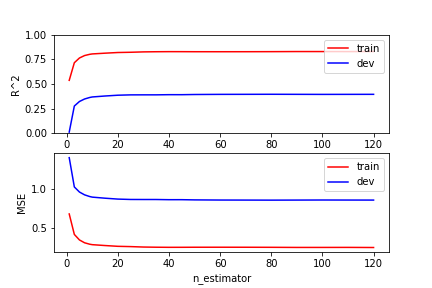
\includegraphics[width=1.2\linewidth, height=0.4\textheight, keepaspectratio]{../plots/RandomForest_nestimator.png}
	\caption{grid search on number of estimators}
	\end{minipage}
	\hfill
	\begin{minipage}[b]{0.4\textwidth}
	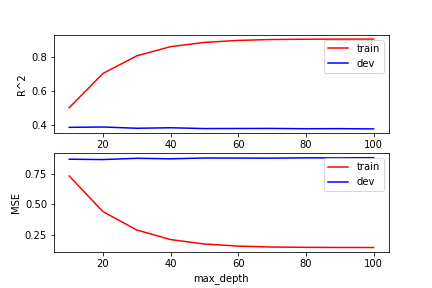
\includegraphics[width=1.2\linewidth, height=0.4\textheight, keepaspectratio]{../plots/RandomForest_maxdepth_tree1.png}
	\caption{grid search on max depth of tree}
	\end{minipage}
	
	\label{fig:feature_imp}
\end{figure}

Another successful model is Random Forest which achieved 0.44 $R^2$ score. This model is compatible with Lightgbm with its accuracy. Other models performed well but did not achieved higher accuracy. 

\begin{figure}
	\centering
	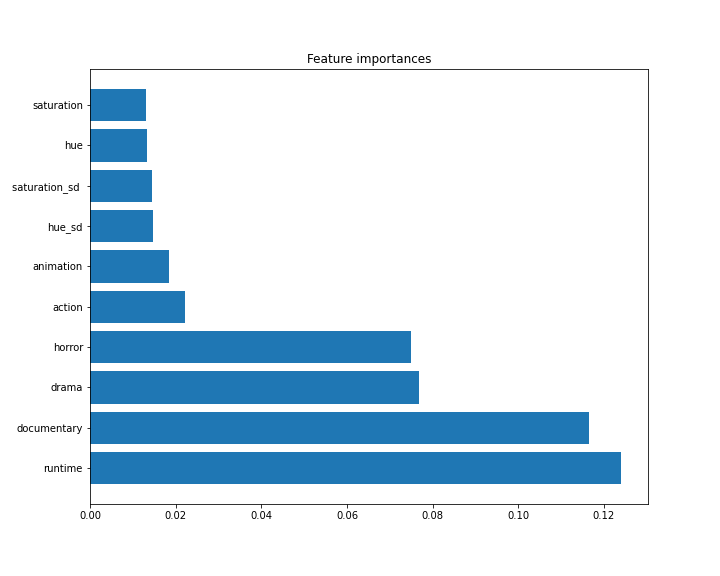
\includegraphics[width=1\linewidth, height=0.4\textheight, keepaspectratio]{../plots/feature_importancvce.png}
	\caption{Feature importance}
	\label{fig:feature_imp}
\end{figure}

\subsection{Hyperparameter tuning}
In the field of Machine Learning one of the things which helps to achieve higher accuracy is hyperparameter tuning. There are a lot of techniques  for this: grid search, hyperopt, random search, gradient-based optimization and etc.. In the case of Lightgbm we have chosen hyperopt and it achieved best score. In Random Forest we have chosen type of grid search, as it trains not very quickly and also its performance is good. In Figure 1 we can see the result of accuracy when searching a best number of estimators in trees and we can see that starting from the 16 it is not improve so much. Moreover, in Figure 2 we can see the search result of max depth of trees and in this case also it is enough to have 32 max depth. 

\subsection{Feature Importance}
It is important question that which parameters affected the most on the prediction of IMDB score. For that we have taken the most important features from Random Forest Regressor and in Figure 3 we can see that runtime affects greatly. The reason could be that people do not like very long or very short movies. Another important feature is documentary genre which is agreeable, as people fun of watching movies which are more realistic. 

\subsection{Classification}
We have also tried to discretized IMDB scores and try to classify movies by their scores. As in [1] we have chosen 5, 10  and 20 classes. In Table 5 we can see the comparison of classification and regression. It is clear from the table that classification MSE is bigger than regression MSE. So, for this problem it is not classification is not working well and regression gives the best score in the sense of MSE. 

\begin{table}
  \caption{Classification vs Regression}
  \label{cls_vs_reg}
  \centering
  \begin{tabular}{lllll}
    \toprule
    Method & cls 5 MSE & cls 10 MSE & cls 20 MSE & reg MSE   \\
    \midrule
    Ridge Regression  & 1.70 & 1.34  & 1.25 & 0.98    \\
    Decision Tree & 1.52 & 1.04 & 1.03 & 0.91 \\
    Random Forest & 0.84 & 0.83  & 0.83 & 0.82 \\
    XGBoost   &1.50 & 1.14  & 1.09 & 0.83 \\
    SVR  & 1.63 & 1.31 & 1.29 & 0.92 \\
        \bottomrule
  \end{tabular}
\end{table}



\section{Conclusion and Future Work}

In this paper we have show some model's performance by predicting IMDB movie rating based on the information available before theatrical release. It is evident that using only that information we cannot get higher accuracy as a lot of information is missing. However, ML methods performed well on this case and the best models error is 0.8 on the test is which is very better than any other existing approaches. 

\section*{References}
\label{reference}

\small

[1] Yichen Yang et al., {\it "Predicting Movie Ratings with Multimodal Data"},
\url{http://cs229.stanford.edu/proj2019aut/data/assignment_308832_raw/26260680.pdf}.

[2] Y. J. Lim and Y. W. Teh, {\it "Variational bayesian approach to movie rating prediction"}  Proceedings of KDD Cup and Workshop, vol. 7, 2007, pp. 15–21.

[3] KaggleInc, {\it “Movie genre from its poster,”} 
\url{https://www.kaggle.com/neha1703/movie-genre-from-its-poster} .

[4] Kaggle, {\it “The movies dataset,” } \url{https://www.kaggle.com/rounakbanik/the-movies-dataset} .

[5] F. B. Moghaddam, M. Elahi, R. Hosseini, C. Trattner, and M. Tkalciˇ c, {\it“Predicting movie popularity and ratings with visual features,” } in 2019 14th International Workshop on Semantic and Social Media Adaptation and Personalization (SMAP). IEEE, 2019, pp. 1–6.

\end{document}